\documentclass[11pt]{report}
\usepackage[margin=1in]{geometry}
\usepackage{pgfplots}
\usepackage{helvet}
\renewcommand{\familydefault}{\sfdefault}

\usepackage{titlesec}

\titleformat{\chapter}{\LARGE\bfseries}{\thechapter.\ }{0em}{}

\usepackage{tikz}
\usetikzlibrary{arrows.meta}

\begin{document}

\title{Performance Evaluation of UNSWBook}
\author{Callum Bannister \and Jerome Samir \and Peter Bishay \and 
Aaron Quan \and Waseem Sajeev}
\date{\today}
\maketitle

\tableofcontents

\chapter{Introduction}
Maintaining quality of service under heavy usage is essential for any web application that expects
a large amount of concurrent users. As there is currently no demand for an asocial media platform,
we have performed a series of experiments on a selection of functions of our UNSWBook application to obtain data on performance degradation as the number of simultaneous users increases. We present the methodology; what functions were tested and what hardware were they tested on. Then, we present results of the experiment, an analysis of the results, and the conclusions to be drawn.  

\chapter{Application Details}

We looked at four basic functionalities of UNSWBook for performance under pressure. They are as follows:

\begin{enumerate}
\item{User login}
\item{Searching for friends}
\item{Adding a friend}
\item{Posting a message}
\end{enumerate}

For each of these functions, we will explain the implementation and what database interactions were required, in order to give context to the performance data in Chapter 3.

\section{User Login}

The user submits their username and password with a POST request. The request body is passed to
the \emph{Login} servlet's doPost method, where we perform initial validation of the input, checking that the required fields exist. \\

Then, we construct the DAO object for a User. We make a single query to the database to check that a non-admin user with the name and password exists, and we retrieve their unique id and whether or not they are banned. Then, we route the user to either the login page, or their home page, returning an error message where necessary. 
\begin{figure}[!htb]
\caption{Control Flow for Login}
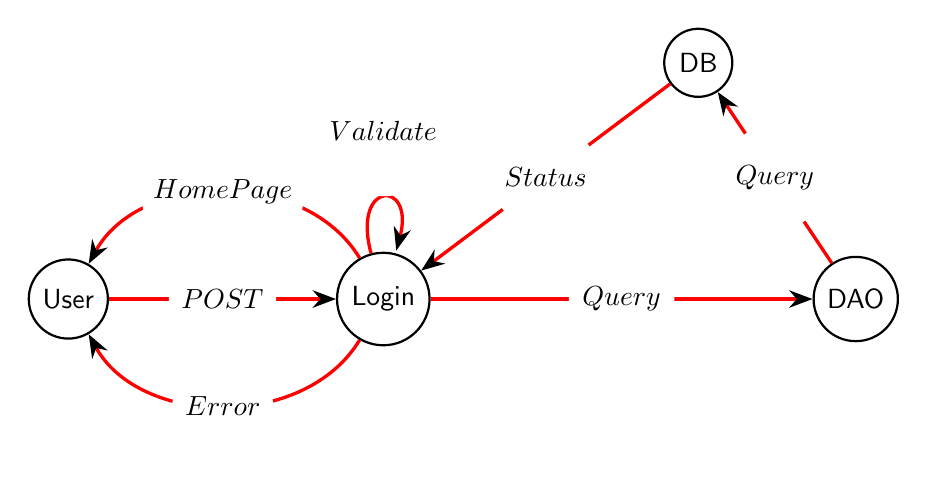
\begin{tikzpicture}
\begin{scope}[every node/.style={circle,thick,draw}]
    \node (User) at (0,0) {User};
    \node (Login) at (4,0) {Login};
    \node (UserDao) at (10, 0) {DAO};
    \node (Database) at (8,3) {DB};
\end{scope}

\begin{scope}[>={Stealth[black]},
              every node/.style={fill=white,circle},
              every edge/.style={draw=red,very thick}]
    \path [->] (User) edge node {$POST$} (Login);
    \path [->] (Login) edge[loop above] node {$Validate$} (Login);
    \path [->] (Login) edge node {$Query$} (UserDao);
    \path [->] (UserDao) edge node {$Query$} (Database);
    \path [->] (Database) edge node {$Status$} (Login);
    \path [->] (Login) edge[bend right=60] node {$Home Page$} (User);
    \path [->] (Login) edge[bend left=60] node {$Error$} (User);
\end{scope}
\end{tikzpicture}
\end{figure}

\section{Search}
In this section we describe only the basic search functionality. We expect that the advanced search to be used relatively infrequently, so optimisation of that function would be of secondary priority. \\

As before, the user submits the search query information via POST, getting routed to the appropriate method in the \emph{Search} servlet. First, we construct a DAO object for the current logged in user, querying the database to obtain their information. Then, we construct a second DAO object, and use it to retrieve a list of users whose username contains the submitted string. We set this as an attribute, and forward the request onto $results.jsp$. 

\begin{figure}[!htb]
\caption{Control Flow for Search}
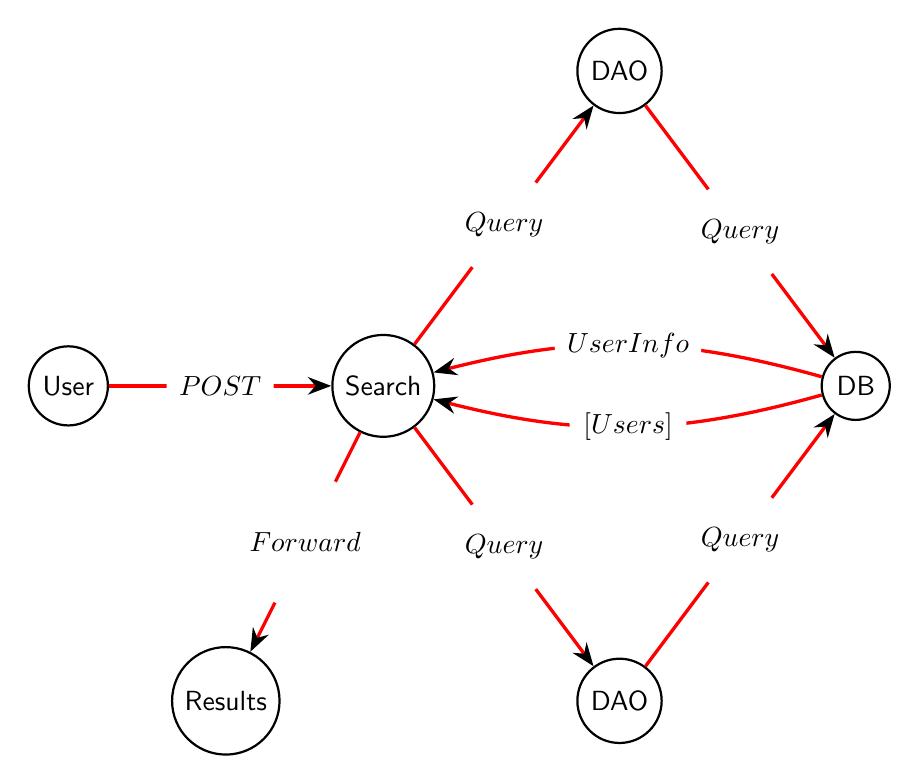
\begin{tikzpicture}
\begin{scope}[every node/.style={circle,thick,draw}]
    \node (u) at (0,0) {User};
    \node (r) at (2,-4) {Results};
    \node (s) at (4,0) {Search};
    \node (ud1) at (7, 4) {DAO};
    \node (ud2) at (7,-4) {DAO};
    \node (db) at (10, 0) {DB};
\end{scope}

\begin{scope}[>={Stealth[black]},
              every node/.style={fill=white,circle},
              every edge/.style={draw=red,very thick}]
    \path [->] (u) edge node {$POST$} (s);
    \path [->] (s) edge node {$Query$} (ud1);
    \path [->] (ud1) edge node {$Query$} (db);
    \path [->] (db) edge[bend right=15] node {$User Info$} (s);
    \path [->] (s) edge node {$Query$} (ud2);
    \path [->] (ud2) edge node {$Query$} (db);
    \path [->] (db) edge[bend left=15] node {$[Users]$} (s);
    \path [->] (s) edge node {$Forward$} (r);
\end{scope}
\end{tikzpicture}
\end{figure}

\section{Adding a friend}
Although adding a friend consists of two operations, the need for a confirmation email to link the two makes measuring them as a conjoined unit unrealistic. Instead, we present only the sending of a friend request. \\

The friend request submits the user id for the requester and the requestee, dispatched to the \emph{FriendReq} servlet. As was the case for \emph{Login}, we perform simple validation of the parameters. Then, we look up the requestee by their id, constructing the DAO and performing the query to the database through it. \\

We add a table to the \emph{friends} database, with the confirmed flag set to $false$, requiring a second query. Afterwards, we extract their email, and send a message containing the appropriate link to confirm the friend request. 

\begin{figure}[!htb]
\caption{Control Flow for Adding a Friend}
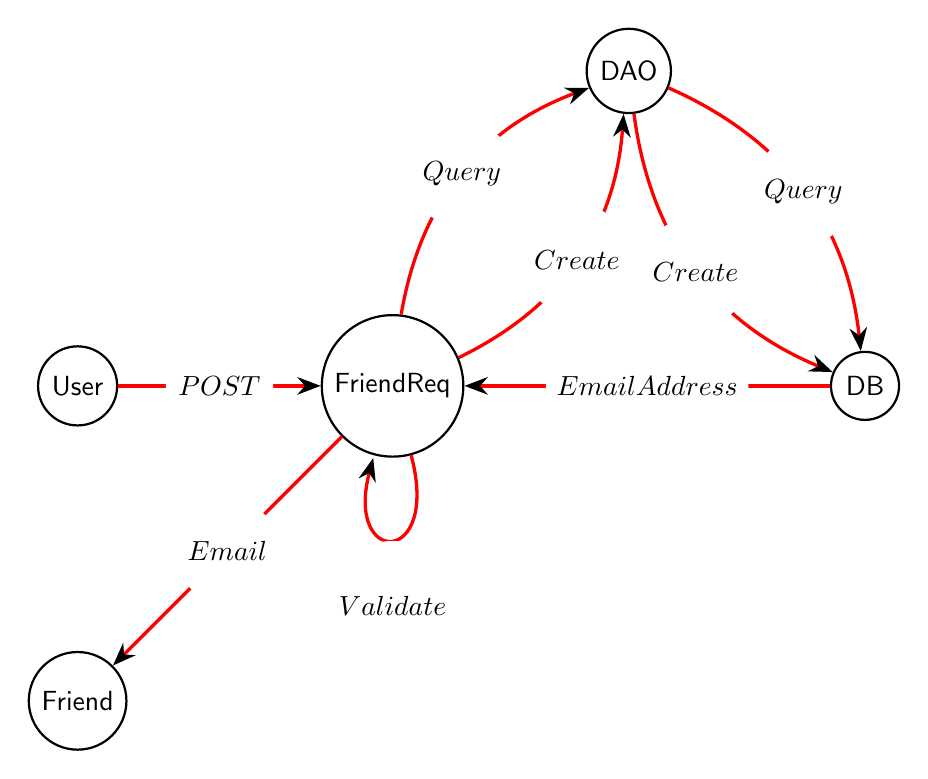
\begin{tikzpicture}
\begin{scope}[every node/.style={circle,thick,draw}]
    \node (u) at (0,0) {User};
    \node (f) at (0,-4) {Friend};
    \node (s) at (4,0) {FriendReq};
    \node (ud) at (7, 4) {DAO};
    \node (db) at (10, 0) {DB};
\end{scope}

\begin{scope}[>={Stealth[black]},
              every node/.style={fill=white,circle},
              every edge/.style={draw=red,very thick}]
    \path [->] (u) edge node {$POST$} (s);
     \path [->] (s) edge[loop below] node {$Validate$} (s);
    \path [->] (s) edge[bend left] node {$Query$} (ud);
    \path [->] (ud) edge[bend left] node {$Query$} (db);
    \path [->] (db) edge node {$Email Address$} (s);
    \path [->] (s) edge[bend right] node {$Create$} (ud);
    \path [->] (ud) edge[bend right] node {$Create$} (db);
    \path [->] (s) edge node {$Email$} (f);
\end{scope}
\end{tikzpicture}
\end{figure}

\section{Posting a message}
Unlike the other operations, the user posts a message by sending a GET request. This is routed to the \emph{Post} servlet, where we once again perform simple validation on the input. We construct the DAO object and look up the currently logged in user as before. We then create a \emph{post} DAO object, and use it to create the appropriate table in the database.

\begin{figure}[!htb]
\caption{Control Flow for Posting a Message}
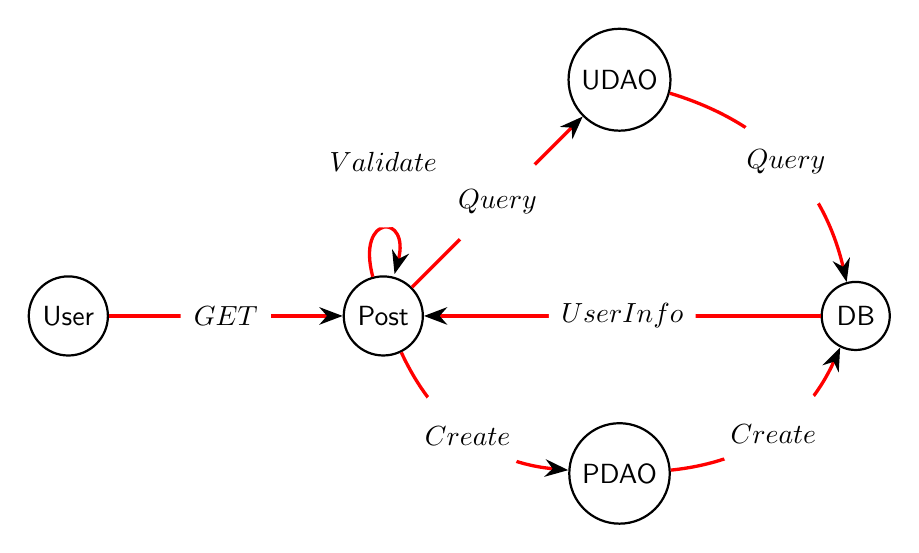
\begin{tikzpicture}
\begin{scope}[every node/.style={circle,thick,draw}]
    \node (u) at (0,0) {User};
    \node (s) at (4,0) {Post};
    \node (ud) at (7, 3) {UDAO};
    \node (pd) at (7,-2) {PDAO};
    \node (db) at (10, 0) {DB};
\end{scope}

\begin{scope}[>={Stealth[black]},
              every node/.style={fill=white,circle},
              every edge/.style={draw=red,very thick}]
    \path [->] (u) edge node {$GET$} (s);
    \path [->] (s) edge[loop above] node {$Validate$} (s);
    \path [->] (s) edge node {$Query$} (ud);
    \path [->] (ud) edge[bend left] node {$Query$} (db);
    \path [->] (db) edge node {$User Info$} (s);
    \path [->] (s) edge[bend right] node {$Create$} (pd);
    \path [->] (pd) edge[bend right] node {$Create$} (db);
\end{scope}
\end{tikzpicture}
\end{figure}

\chapter{Test Setup}
In this chapter we present the hardware, setup, and experimental procedure that we used to obtain the data.

\section{Server}

The application server had the following hardware specifications:
\begin{table}[htp]
\caption{Server Hardware}
\begin{center}
\begin{tabular}{l | c}
Hardware & Specification \\ \hline
HDD & 16 GB 1600 MHz DDR3 \\
RAM & 16GB \\ 
CPU & 2.3 GHz Intel Core i7 \\
\end{tabular}
\end{center}
\label{default}
\end{table}%

The machine was running macOS Sierra 10.12.4, with JVM Version 1.7.0. We used Tomcat 7.0.42 as our server, and Apache Derby 10.9.1 as our database. To maximise the accuracy of our results the only user processes on the machine were the Tomcat and Derby servers. \\

The connection pool size was kept at the default for the jdbc driver (a \emph{maximum} of 100 and \emph{minimum} of 10). We did not predict that manipulating this value would lead to significantly different results.

\section{Client}

The client had the following hardware specifications:
\begin{table}[htp]
\caption{Client Hardware}
\begin{center}
\begin{tabular}{l | c}
Hardware & Specification \\ \hline
HDD & 16 GB 1600 MHz DDR3 \\
RAM & 16GB \\ 
CPU & 2.3 GHz Intel Core i7 \\
\end{tabular}
\end{center}
\label{default}
\end{table}%

As with the server machine, extraneous processes were kept to a minimum. Both the client and server were on the same LAN, minimising factors unrelated to the performance of UNSWBook from affecting the results.

\section{Experimental Method}
We constructed our experiment to simulate the following scenario:

\begin{enumerate}
\item{A user logs in, searches for a new friend, adds them, and posts a message to acknowledge their new friendship}
\end{enumerate}

We added a delay of five seconds between each user action. We tested this scenario for increasing numbers of concurrent users: 5,10,20,40,50,75,100 and 200. Before each test attempt, we cleared the database of any existing posts and/or friends, in order to keep those factors constant. \\

However, at 200 requests, we ran into authentication errors when trying to send out emails for friend requests, distorting the data. While this did not indicate a performance issue in the conventional sense, it demonstrated an issue that would not become apparent without placing the application under heavy load. 

\chapter{Results}
\section{Data}
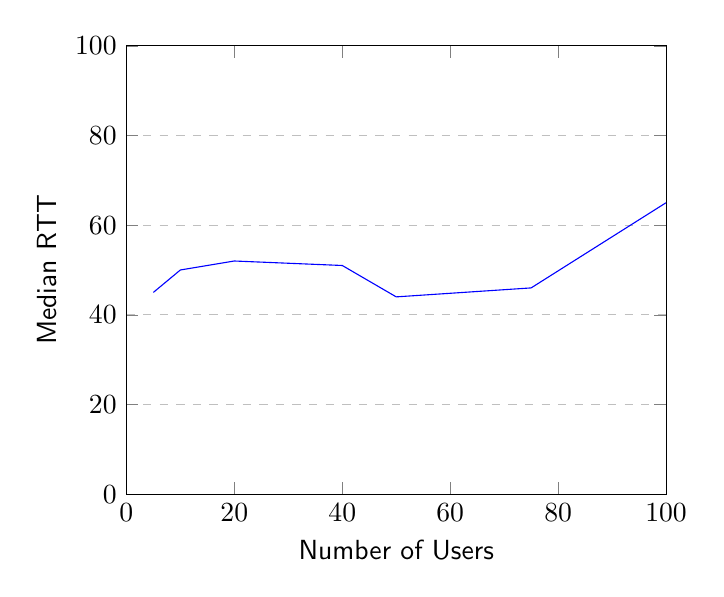
\begin{tikzpicture}
\begin{axis}[
    xlabel={Number of Users},
    ylabel={Median RTT},
    xmin=0, xmax=100,
    ymin=0, ymax=100,
    xtick={0,20,40,60,80,100},
    ytick={0,20,40,60,80,100},
    legend pos=north west,
    ymajorgrids=true,
    grid style=dashed,
]
 
\addplot[
    color=blue,
    mark=circle,
    ]
    coordinates {
    (5, 45)(10,50)(20,52)(40,51)(50, 44)(75, 46)(100, 65)
    };
 
\end{axis}
\end{tikzpicture}

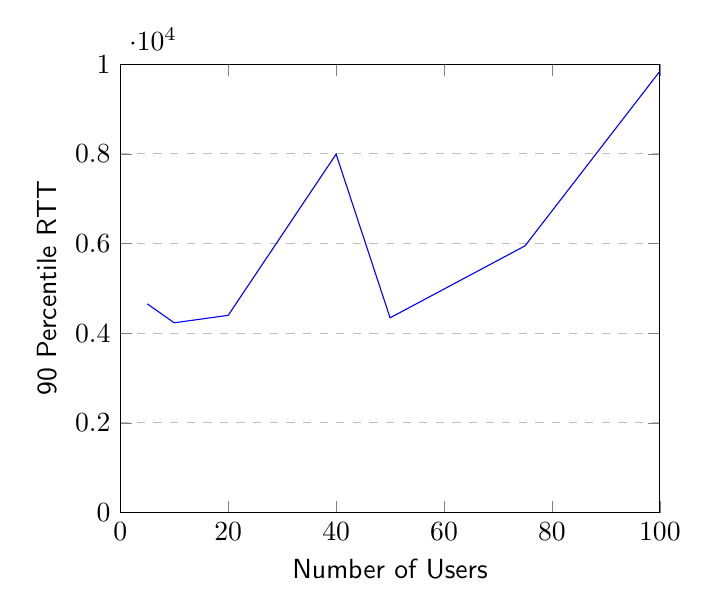
\begin{tikzpicture}
\begin{axis}[
    xlabel={Number of Users},
    ylabel={90 Percentile RTT},
    xmin=0, xmax=100,
    ymin=0, ymax=10000,
    xtick={0,20,40,60,80,100},
    ytick={0,2000,4000,6000,8000,10000},
    legend pos=north west,
    ymajorgrids=true,
    grid style=dashed,
]
 
\addplot[
    color=blue,
    mark=circle,
    ]
    coordinates {
    (5, 4655)(10,4232)(20,4398)(40,7994)(50, 4343)(75, 5947)(100, 9844)
    };
 
\end{axis}
\end{tikzpicture}

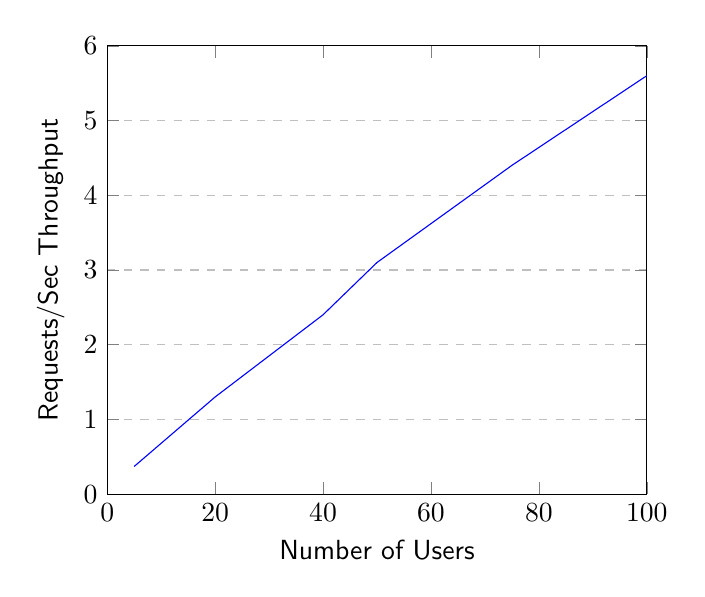
\begin{tikzpicture}
\begin{axis}[
    xlabel={Number of Users},
    ylabel={Requests/Sec Throughput},
    xmin=0, xmax=100,
    ymin=0, ymax=6,
    xtick={0,20,40,60,80,100},
    ytick={0,1,2,3,4,5,6},
    legend pos=north west,
    ymajorgrids=true,
    grid style=dashed,
]
 
\addplot[
    color=blue,
    mark=circle,
    ]
    coordinates {
    (5, 0.37)(10,0.68)(20,1.3)(40,2.4)(50, 3.1)(75, 4.4)(100, 5.6)
    };
 
\end{axis}
\end{tikzpicture}

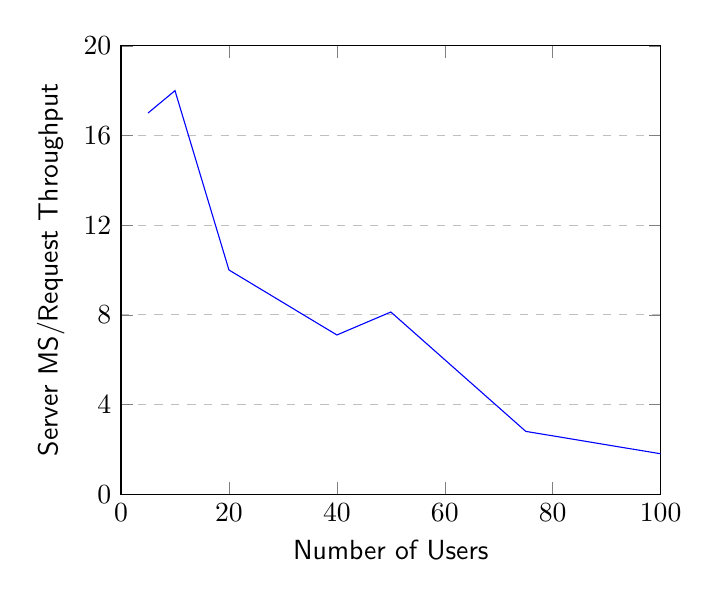
\begin{tikzpicture}
\begin{axis}[
    xlabel={Number of Users},
    ylabel={Server MS/Request Throughput},
    xmin=0, xmax=100,
    ymin=0, ymax=20,
    xtick={0,20,40,60,80,100},
    ytick={0,4,8,12,16,20},
    legend pos=north west,
    ymajorgrids=true,
    grid style=dashed,
]
 
\addplot[
    color=blue,
    mark=circle,
    ]
    coordinates {
    (5, 17)(10,18)(20,10)(40,7.1)(50, 8.125)(75, 2.8)(100, 1.8)
    };
 
\end{axis}
\end{tikzpicture}

\section{Analysis}
For the bounds we were able to test, we noticed no degradation of the application performance. Aside from the email errors, it appeared as though we were able to support at least 200 users simultaneously. The throughput behaves as expected. \\

We observed that adding a friend caused the largest amount of delay, due to the sending of an email in order to confirm the friend request. A probable performance improvement would be to off-load the work into a queue or pool for later processing, and return to the user immediately, as the immediate sending of a friend request would be of a low priority compared to general responsiveness. \\


Unfortunately, we were not able to test UNSWBook on higher loads, due to the errors we found with sending friend requests.This indicates more work needs to be done on the functionality of the application under high load, rather than just responsiveness. Despite that, performance seemed good on what we tested - most operations require only one or two database calls. 

\chapter{Conclusion}
We were able to gather some useful data on deploying UNSWBook under a realistic load environment. While the performance of our application held up, we found that the friend request functionality began to show errors under a high load. This indicates that the most productive area to focus on for improvement would be fixing this functionality. 
\end{document}
